\subsection{Behavioral Coverage and Report Compactness}
\label{sec:analysiscoverage}

\begin{figure}[ht]
\centering
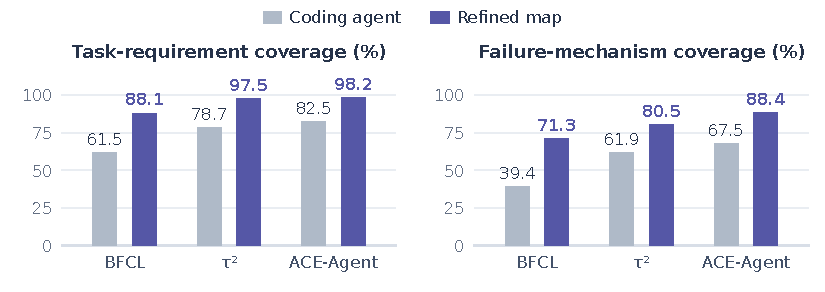
\includegraphics[width=\linewidth]{figures/analysis_coverage.pdf}
\caption{Task and failure coverage of the coding-agent reports and refined map
under the final paired evaluation. Report lengths and historical grades are
retained in Appendix~\ref{app:analysiscoverage}.}
\label{fig:analysiscoverage}
\end{figure}


We now test whether a structured analysis process reduces the information loss
identified in Section~\ref{sec:coveragegap}. On the same 1,692 frozen initial
Qwen3-8B public-eval trajectories, we compare the fixed coding-agent reports
(Astra/high) with a standalone, coverage-checked refinement of the behavioral
map (GPT-5.5/high). The refinement analyzes complete task evidence, consolidates
shared mechanisms, and checks the compact report for omitted conditions. It
receives neither the reference labels nor the coding agent's report prose.
We extend the same protocol to 243 initial public-eval trajectories of
Qwen3-4B-Instruct-2507 on AppWorld.

\textbf{Measure retained meaning, not compression alone.}\quad
Frozen, source-grounded reference units describe task requirements and failure
mechanisms. An LLM judge scores anonymized report pairs as full, partial,
missing, or contradicted. Only full preservation of the mechanism and its
consequential scope or dependency receives credit. We average units within
each task and then tasks within each corpus; word count separately measures
compactness. References are generated before seeing candidate reports, not
inferred from either method's preferred categories. Appendix~\ref{app:analysiscoverage}
gives the protocol, grading variability, costs, and spot audit.

\textbf{Higher coverage in shorter reports.}\quad
The refined map reaches 88.1--99.5\% task-requirement coverage and 71.3--88.4\%
failure-mechanism coverage, while using 12--29\% fewer words
(Figure~\ref{fig:analysiscoverage}a). It exceeds the paired
grades of the coding-agent reports on all four corpora; the ordering
also holds under subset--family-balanced aggregation. A concrete ACE example
shows why this is more than naming more error types: an inbox-cleanup timeout
label omits the user-authorization--deletion--retry dependency, which the
refined report preserves. Both graders support partial versus full coverage
for that example. Not every case improves; partially preserved mechanisms and
other collapsed distinctions are documented in Appendix~\ref{app:analysiscoverage}.

These development-set results support more comprehensive, compact behavioral
analysis in this setting. They do not isolate the hierarchy from the added
coverage checks, match backbones or computation, or establish downstream RL
gains. The diagnostic is separate from the historical 4B training runs.
